\documentclass[a4paper,10pt]{report}
\usepackage[utf8x]{inputenc}
\usepackage[french]{babel}
\usepackage[letterpaper]{geometry}
\geometry{verbose,tmargin=2cm,bmargin=2cm,lmargin=2cm,rmargin=2cm}
\usepackage{graphicx} 
\usepackage{color}
\setcounter{secnumdepth}{3}
\setcounter{tocdepth}{3}
\usepackage{amsmath}
\usepackage{amssymb}
\usepackage{mathptmx}
\usepackage{ifthen}
\usepackage[T1]{fontenc}
\usepackage{float}
\usepackage{textcomp}
\usepackage{setspace}
\usepackage{listings}
\usepackage{array}
\usepackage[unicode=true, pdfusetitle, bookmarks=true,bookmarksnumbered=false,bookmarksopen=false,
breaklinks=false,pdfborder={0 0 0},backref=false,colorlinks=false,pdfauthor={St\'ephanie Ouillon -- Tiezhen Wang}]{hyperref}

\definecolor{colKeys}{rgb}{0,0,1} 
\definecolor{colIdentifier}{rgb}{0,0,0} 
\definecolor{colComments}{rgb}{0,0.5,1} 
\definecolor{colString}{rgb}{0.6,0.1,0.1} 

\lstset{%configuration de listings 
float=hbp,% 
basicstyle=\ttfamily\small, % 
identifierstyle=\color{colIdentifier}, % 
keywordstyle=\color{colKeys}, % 
stringstyle=\color{colString}, % 
commentstyle=\color{colComments}, % 
columns=flexible, % 
tabsize=2, % 
frame=trBL, % 
frameround=tttt, % 
extendedchars=true, % 
showspaces=false, % 
showstringspaces=false, % 
numbers=left, % 
numberstyle=\tiny, % 
breaklines=true, % 
breakautoindent=true, % 
captionpos=b,% 
xrightmargin=+0cm, % 
xleftmargin=+0cm
}

\AtBeginDocument{
  \def\labelitemi{\(\bullet\)}
}

% Title Page
\title{Integration of the "trains protocol" to the middleware JGroups \\ Project of last year}
\author{St\'ephanie Ouillon -- Tiezhen Wang   \\ \\ \\ \\ \\ \\ 
\includegraphics[scale=0.3]{img/int.jpg}}
\date{\today}


\begin{document}
\maketitle

\tableofcontents

\chapter{Introduction}

The trains protocol is a uniform and totally-ordered broadcast protocol \footnote{ Défago, X., Schiper, A. et Urbán, P. (2004). Total order broadcast and multicast algorithms : Taxonomy and survey. ACM Comput. Surv., 36:372?421}.
It is designed to be a throughput-efficient protocol, especially for short messages (100 bytes or lower)\footnote{M. Simatic. Communication et partage de données dans les systèmes répartis (Data communication and data sharing in distributed system, in French). PhD thesis, École Doctorale ÉDITE, October 2012 (available at http://www-public.it-sudparis.eu/~simatic/Recherche/Publications/theseSimatic.pdf)}.
So far, the trains protocol has been implemented in C during the year 2012 at T\'el\'ecom SudParis.

\section{Integration with JGroups}

JGroups\cite{jgroups} is a reliable multicast system written in Java language. It has a flexible protocol stack which allows developpers to 
adapt it to their application requirements.
The primary goal of this project is to provide JGroups with an implementation of the trains protocol.

JGroups adds a "grouping" layer over a transport protocol, internally keeping a list of participants. 
It can be used to create groups of processes whose members can send messages to each other\cite{wikipedia}.
More importantly, when a member joins or leaves, JGroups takes care of transfering the current state of the group so that the new member
gets the history of the messages that were sent while it was offline.

Because the initial C implementation of the trains protocol doesn't implement this state transfer, integrating the protocol to JGroups
would allow to test the default state transfer protocol of JGroups with the protocol. 

\section{Global Roadmap}

The steps of this projet will be the following ones: 

\begin{enumerate}
  \item \textbf{Java implementation:} the trains protocol needs to be implemented in Java in order to be integrated to JGroups
  \item \textbf{Integration in the protocol stack of JGroups}
  \item \textbf{State transfer}: testing the state transfer feature of JGroups with the trains protocol
  \item \textbf{Performance and application:} using JGroups and the trains protocol in a real use-case and study performances
\end{enumerate}

\begin{center}
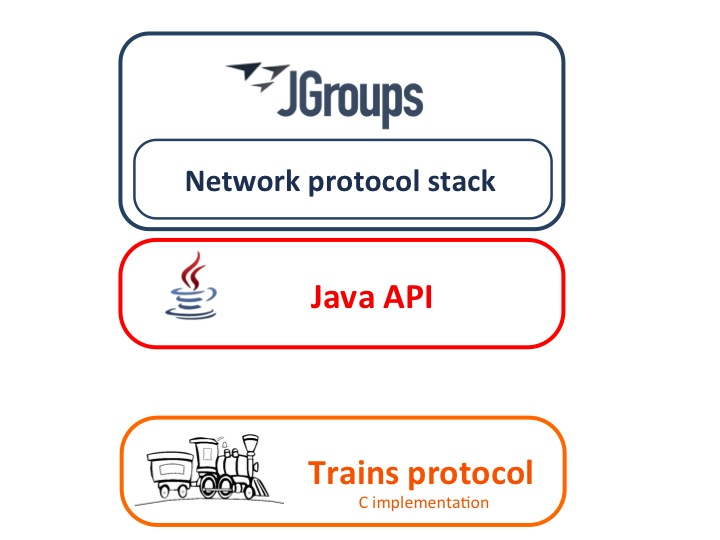
\includegraphics[scale=0.4]{img/stack.jpg}
\end{center}

\section{A closer look at the trains protocol}

\subsection{Brief introduction to the protocol}

\textit{The following part is freely inspired by the chapter 4 entitled "The trains protocol" of the thesis of Michel Simatic (in French)\footnote{\textit{Ibid}}}.\\

The trains protocol comes from the idea of the train protocol of [Cristien, 1991]. Briefly explained, one or several trains of messages
run between the participating processes which are distributed on a virtual ring. The following sections approximatively exposes some of the
notions explained in the thesis.\\


\textbf{System model:} The trains protocol is meant to be run on a small cluster of homogeneous machines connected on a local network (typically with a switch). Each machine
can run one or several processes participating to the trains protocol. These processes are distributed on a virtual ring. Each processus is then
connected via TCP to the previous and the following process on this ring. The messages run in the same way.
Given the simplicity of the implemented communications, the homogeneous environment and the low latency of the network, the processus at the other end of the connection is considered to be failing if the TCP connection fails.\\


\textbf{Some definitions:}\\ 
A \textit{circuit of trains} is the virtual ring on which the processes participating to the 
trains protocol are distributed.\\
The \textit{train} is a token running on the circuit. It carries the messages to be broadcasted inside \textit{wagons}.
When a processus wants to broadcast a message, it adds it to a wagon (a data structure) and then waits to receive the first passing train/token to add
this wagon at the end of the train.\\
The \textit{address} of a process is a unique identifiant for the given process in the trains protocol.

\subsection{State of the implementation in C}

The trains protocol is completely implemented in C - except the feature of state transfer - and some performance tests have been made.
The documentation is available through doxygen.
What is important to remember is that this version of the trains protocol has been developped and tested on Linux. It requires 
some work to make it compatible with operating systems such as Windows and Mac OS X. We'll come back to this issue at the chapter 2, 
section 4 of this document.\\

The user can use the trains protocol by loading the libtrains.so library and interact with a set of functions:
\begin{itemize}
  \item interface.c: trInit() to initialize the process, trTerminate()
  \item applicationMessage.c: newmsg() to create a new message, utoBroadcast() to send it\\
\end{itemize}


The code of this implementation is available on GitHub\footnote{TrainsProtocol depository: https:/github/simatic/TrainsProtocol}.
A tutorial is also online\footnote{Tutorial: http://www-tp-ext.it-sudparis.eu/\~foltz\_r/trainsTutorial.html}.

A basic use of the protocol is implemented in some file tests, particularly in TrainsProtocol/tests/integration/basic.
So here is the skeleton of a basic program using the train protocol:\\

\lstset{language=C}
\lstset{commentstyle=\textit} 
\begin{lstlisting}
#include "trains.h"
#include "errorTrains.h"

void callbackCircuitChange(circuitView *cp){
  /* When a process joins or leaves the circuit, 
   * the code runs the instructions of this callback */
}

void callbackUtoDeliver(address sender, message *mp){
  /* When a message is received by the process,
   * the system executes the instructions of this callback */
}

int main(int argc, char *argv[]){
  
  /* Initialize the protocol and provide it with the callback functions
   * defined by the user */
  trInit(0, 0, 0, 0, callbackCircuitChange, callbackUtoDeliver);

  /* Create a new message to be sent (allocation in a wagon) */
  message *mp = newmsg(PAYLOAD_SIZE);

  /* Fill in the content of the message */
  *(mp->payload) = content;

  /* Broadcast the message (put it in the train when it comes) */
  utoBroadcast(mp)

  /* Terminates the train protocol (actually returns only 0)*/
  rc = trTerminate();
}
\end{lstlisting} 

This is the starting point to design the Java API for the trains protocol. Let's consider more precisely what this
implementation has to perform.

\chapter{Java implementation of the trains protocol}

\section{Designing the API}

The Java API of the train protocol is designed to be used in 2 types of context:
\begin{enumerate}
  \item Implementing the trains protocol in a custom Java program
  \item Integrating the trains protocol in the network protocol stack of JGroups\\
\end{enumerate}

Therefore, the Java API needs to be the more generalized it can be but it has still to fit with the code environment of JGroups.

\subsection{Using the Java Native Interface (JNI)}

Implementing the trains protocol in C gave the ability to tune the code to reach good performance timings and optimization.
Given the work that has been already done on this implementation and the limited amount of time of this current project, 
it was decided to re-use this code. Calling C functions from the Java Virtual Machine is possible with the Java Native Interface (JNI).
The Java program running in a JVM and the \textit{native} C code can interact together, pass values from one to each other, call functions from one or the another
language. As a matter of fact, speaking of a "Java implementation" of the trains protocol is a inexact but we'll still use this expression
meaning the Java interface of the trains protocol.\\

\begin{center}
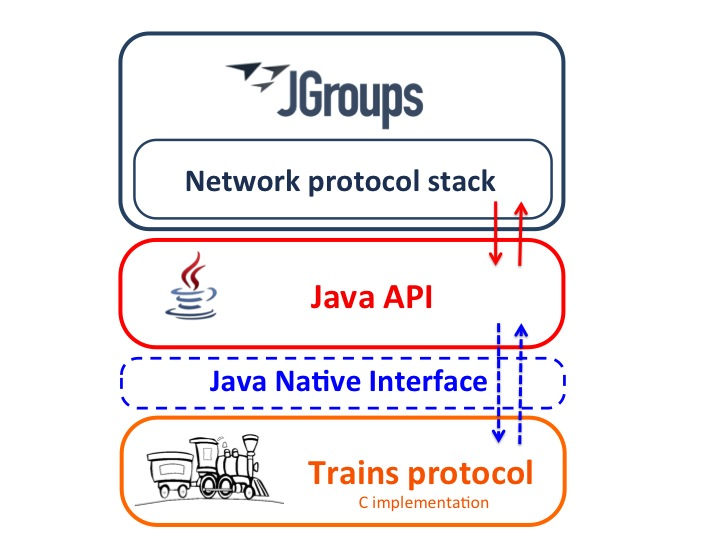
\includegraphics[scale=0.4]{img/stackJNI.jpg}
\end{center}

Here are the basics of using JNI in Java, i.e. calling C functions in a Java program.\\

The first step is to implement a class that will be the interface to interact with the native code. This class:
\begin{itemize}
  \item loads the native library
  \item declares the prototypes of the native functions that will be called from the JVM and that are implemented in the loaded library
   \item writes Java wrappers to call theses functions from Java.\\
\end{itemize}

\lstset{language=java}
\lstset{commentstyle=\textit} 
\begin{lstlisting}
public class Interface{

  /* Declaration of the prototype of the native function */
  public native int return42();

  public static Interface myInterface(){

    /* Load the native library where return42() is implemented */
    System.loadLibrary("mylibrary");
    Interface myInterface = new Interface();
    return myInterface;
  }

  /* Wrapper for the native function return42() */
  public int Jreturn42(){
    /* Execute the C function and return the result to the JVM */
    return return42();
  }
}
\end{lstlisting}

Then the javah tool generates a header Interface.h for the C implementation of return42():\\
\lstset{language=C}
\lstset{commentstyle=\textit} 
\begin{lstlisting}
/* DO NOT EDIT THIS FILE - it is machine generated */
#include <jni.h>
/* Header for class trains_Interface */

#ifndef _Included_trains_Interface
#define _Included_trains_Interface
#ifdef __cplusplus
extern "C" {
#endif
/*
 * Class:     Interface
 * Method:    return42
 * Signature: (V)I
 */

JNIEXPORT jint JNICALL Java_Interface_return42(JNIEnv *, jobject);

#ifdef __cplusplus
}
#endif
#endif
\end{lstlisting}

Including this header and the header jni.h installed with the JDK, we can code the native function:\\

\lstset{language=C}
\lstset{commentstyle=\textit} 
\begin{lstlisting}
#include <jni.h>
#include Interface.h

JNIEXPORT jint JNICALL Java_Interface_return42(JNIEnv *, jobject){
  return 42
}

\end{lstlisting}

At last, the native library is generated from the C source code. It is worth noticing that the Java code to load the library is: \\
\lstset{language=java}
\lstset{commentstyle=\textit} 
\begin{lstlisting}
System.loadLibrary("mylibrary");
\end{lstlisting}

The library format can vary between ".so" on Linux, ".jnilib" on Mac OS X or ".dll" on Windows but it does not have to be specified to be loaded by the JVM.
Also, it is not necessary - and it is not recommended - to write the full path of the library. It will be exported in an environment variable: LD\_LIBRARY\_PATH on Linux or
DYLD\_LIBRARY\_PATH on OS X.

\subsection{Calling Java code from native code}

It is not enough to be able to call native functions from a Java program. In the trains protocol, each time a change happens on the circuit
or a message is received, the program calls a callback function defined by the programmer.
If the programmer writes his/her program in Java, he/she will write the callback functions in Java, too. So the native code, dealing with
low levels of the protocol - circuit changes and messages reception - have to be able to call Java code.
Fortunetately with JNI, native code can call Java functions as well as the opposite. So the Java programmer won't have to be aware of
what the C program does or to modify it to run the "Java implementation" of the trains protocol.  

\subsection{The C interface}

To use the trains protocol in C, the programmer calls a set of functions defined in 2 files:
\begin{itemize}
  \item \textbf{interface.c:}\\ 

\lstset{language=C}
\lstset{commentstyle=\textit} 
\begin{lstlisting}
#include <stdlib.h>
#include <stdio.h>
#include <pthread.h>
#include <errno.h>

#include "interface.h"
#include "management_addr.h"
#include "iomsg.h"
#include "stateMachine.h"
#include "errorTrains.h"

/**
 * @brief Initialization of trains protocol middleware

 * @param[in] trainsNumber The number of trains on the circuit
 * @param[in] wagonLength The length of the wagons in the trains
 * @param[in] waitNb The number of time to wait
 * @param[in] waitTime The time to wait (in microsecond)
 * @param[in] callbackCircuitChange Function to be called when there is a circuit changed (Arrival or departure of a process)
 * @param[in] callbackUtoDeliver    Function to be called when a message can be uto-delivered by trains protocol
 * @return 0 upon successful completion, or -1 if an error occurred (in which case, @a trErrno is set appropriately)
 */
int trInit(int trainsNumber, int wagonLength, int waitNb, int waitTime,
    CallbackCircuitChange callbackCircuitChange,
    CallbackUtoDeliver callbackUtoDeliver){
}

/**
 * @brief TrainsProtocol version of ERROR_AT_LINE
 * @param[in] status
 * @param[in] errnum
 * @param[in] filename
 * @param[in] linenum
 * @param[in] format
 * @return void
 */
void trError_at_line(int status, int errnum, const char *filename, unsigned int linenum, const char *format){}

/**
 * @brief TrainsProtocol version of perror
 * @param[in] errnum
 * @return void
 */
void trPerror(int errnum){}

int trTerminate(){}
\end{lstlisting}

  \item \textbf{applicationMessage.c:}\\
\lstset{language=C}
\lstset{commentstyle=\textit} 
\begin{lstlisting}
#include <string.h>
#include <stdio.h>
#include "applicationMessage.h"
#include "trains.h"
#include "wagon.h"
#include "msg.h"
#include "advanced_struct.h"
#include "counter.h"
#include "stateMachine.h"

CallbackCircuitChange theCallbackCircuitChange;
CallbackUtoDeliver theCallbackUtoDeliver;

message *newmsg(int payloadSize){}

int utoBroadcast(message *mp){}

...

\end{lstlisting}

\lstset{language=C}
\lstset{commentstyle=\textit} 
\begin{lstlisting}
JNIEXPORT jint JNICALL Java_trains_Interface_utoBroadcast(JNIEnv *, jobject, jobject);
\end{lstlisting}
\end{itemize}

\section{The Java API}

The code of the Java API is available on GitHub\footnote{https://github.com/simatic/TrainsProtocolJava}.

\subsection{UML diagrams}

Here is the UML diagram of the Java API in the package trains.\\

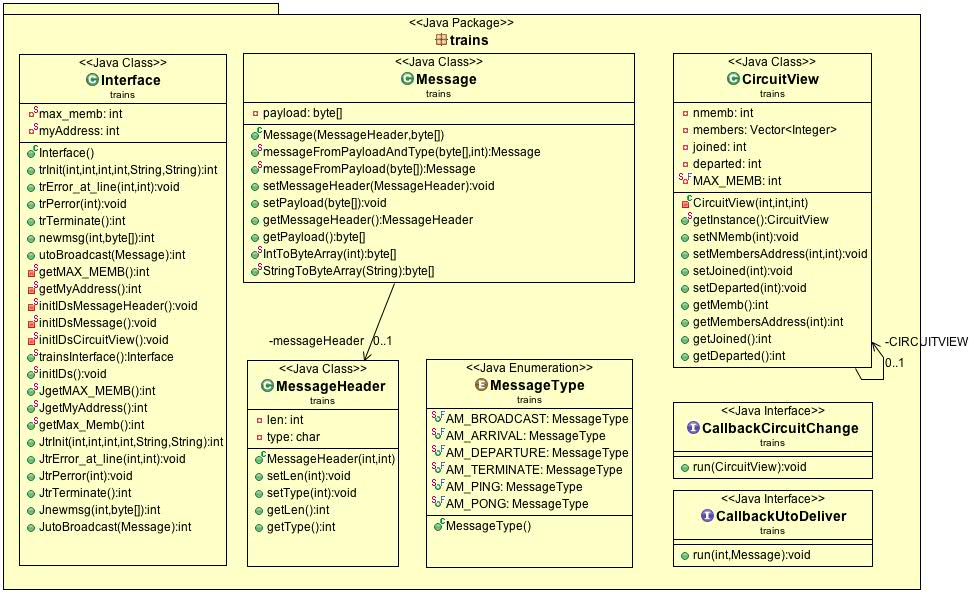
\includegraphics[scale=0.55]{img/trainsInterface.jpg}\\

The following diagram shows how a program can use this interface.\\

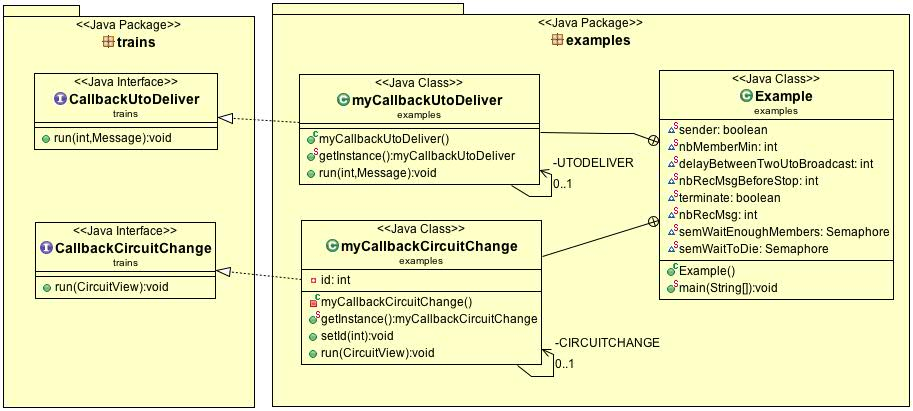
\includegraphics[scale=0.55]{img/example.jpg}\\

\subsection{Some points about the Java API}

Let's talk about some aspects of this API.

The JNI defines a set of C and C++ types that correspond to types in the Java programming language.
e.g.: jint for int, jchar for char, jbyteArray for byte[].
Some structures defined in C - such as application messages, message headers and circuit views - are passed as arguments to the Java 
program. To represent these structures in Java, classes are defined and each attribute is a field of the C structure : MessageHeader, 
Message and CircuitView.

Following the same idea, an enum class was defined to store the values of message types (AM\_BROADCAST, AM\_ARRIVAL, etc): MessageType.\\

In C, trInit() gets two functions which are callbacks: CallbackCircuitChange and CallbackUtoDeliver.
In Java, CallbackCircuitChange and CallbackUtoDeliver are interfaces that are to be implemented by the user. The running code
is defined in a run() method. The classes are instantiated by the native code in utoDeliveries() (in applicationMessage.c).
It is important to notice that these callbacks are meant to be singletons. So when the programmer
declares and implements the classes, he/she needs to declare a getInstance() static factory that will be called from the native code.

\section{Implications of using JNI}

\subsection{Modifications of the initial C API}

\subsection{The JNI environment pointer}

The native code can access the Java Virtual Machine through the JNI environment pointer. This pointer is passed to every function that
implements native code as its first argument.\\

\lstset{language=C}
\lstset{commentstyle=\textit} 
\begin{lstlisting}
JNIEXPORT jint JNICALL Java_trains_Interface_utoBroadcast(JNIEnv *, jobject, jobject);
\end{lstlisting}

The JNI documentation\cite{jnidoc} explains that "A JNIEnv interface pointer is a pointer to thread-local data, which in turn contains a 
pointer to a function table. Every interface function is at a predefined offset in the table."

An important feature is that "The virtual machine is guaranteed to pass the same interface pointer to native method implementation functions called from the same thread. 
However, a native method can be called from different threads, and therefore may be passed different JNIEnv interface pointers. 
Although the interface pointer is thread-local, the doubly indirected JNI function table is shared among multiple threads."
This is an important point to remember, we will come back to it in another subsection.

In the C implementation of the trains protocol, the initialization of the protocol via trInit() launches a new thread to run
utoDeliveries(). utoDeliveries performs a while loop and receives every message from the protocol - arrival, departure, broadcast messages -
and so calls the appropriate callback.\\
 
\lstset{language=C}
\lstset{commentstyle=\textit} 
\begin{lstlisting}

interface.c

int trInit(int trainsNumber, int wagonLength, int waitNb, int waitTime,
    CallbackCircuitChange callbackCircuitChange,
    CallbackUtoDeliver callbackUtoDeliver){

  int rc;
  ...

  rc = pthread_create(&thread, NULL, utoDeliveries, NULL);
  if (rc)
    ERROR_AT_LINE(EXIT_FAILURE, rc, __FILE__, __LINE__, "pthread_create");
  
  ...
}

//
applicationMessage.c


void *utoDeliveries(void *null){
  wiw *wi;
  wagon *w;
  message *mp;
  circuitView cv;
  bool terminate = false;

  do {
    wi = bqueueDequeue(wagonsToDeliver);
    w = wi->p_wagon;

    // We analyze all messages in this wagon
    for (mp = firstMsg(w); mp != NULL ; mp = nextMsg(w, mp)) {
  
      ...

      switch (mp->header.typ) {
          
      ... 

      case AM_BROADCAST:
        (*theCallbackUtoDeliver)(w->header.sender, mp);
        break;
      case AM_ARRIVAL:
        fillCv(&cv, ((payloadArrivalDeparture*) (mp->payload))->circuit);
        cv.cv_joined = ((payloadArrivalDeparture*) (mp->payload))->ad;
        (*theCallbackCircuitChange)(&cv);
        break;
      case AM_DEPARTURE:
        fillCv(&cv, ((payloadArrivalDeparture*) (mp->payload))->circuit);
        cv.cv_departed = ((payloadArrivalDeparture*) (mp->payload))->ad;
        (*theCallbackCircuitChange)(&cv);
        break;
        
      ...

    }
    freeWiw(wi);
  } while (!terminate);

  return NULL ;
}


\end{lstlisting}

In the Java implementation, one sole JVM runs. The JVM calling trInit() to initialize the trains protocol and the JVM executing
the callbacks have to be the same.
JtrInit() is the JNI interface. It receives a JNIenv pointer as a first argument. We'll get and store the JavaVM in a global variable
that will be accessible wherever it needs to be so that the JNIenv pointer can be get and callbacks be run in the same JVM.\\

\lstset{language=C}
\lstset{commentstyle=\textit} 
\begin{lstlisting}

interface.c

JavaVM *jvm;

JNIEXPORT jint JNICALL Java_trains_Interface_trInit(JNIEnv *env, 
    jobject obj, jint trainsNumber, jint wagonLength, jint waitNB, 
    jint waitTime, 
    jstring callbackCircuitChange,
    jstring callbackUtoDeliver){

  ...  
  (*env)->GetJavaVM(env, &jvm);
  ...

}
//
applicationMessage.c

void *utoDeliveries(void *null){

  ...
  /* Get the JNIenv pointer*/
  JNIEnv *JNIenv;
  (*jvm)->AttachCurrentThread(jvm, (void **)&JNIenv, NULL);
  if (*JNIenv == NULL){
    ERROR_AT_LINE(EXIT_FAILURE, 1, __FILE__, __LINE__, "attach the current thread to the JVM");
  }
  ...

}
\end{lstlisting}

\subsection{Caching fields and methods IDs}

When the native code calls Java methods or wants to access Object attributes via setters or getters, it needs to get an identifiant (ID)
for the method or the field.

Obtaining field and method IDs requires symbolic lookups based
    on the name and descriptor of the field or method. Symbolic lookups
    are relatively expensive.
    
    We cache some field IDs and objects in static methods that are called
    when we first load the library (instantiation of Interface.java).
    Doing so, we initialize the field IDs required by a native method before
    the application can have a chance to invoke the native method.
    Therefore, we don't have check to detect whether the IDs have already
    been cached.

\subsection{Performance of JNI field and method operations}

The following lines are from the JNI Sun documentation\footnote{http://192.9.162.55/docs/books/jni/html/fldmeth.html\#30642}.\\

"What are the performance characteristics of accessing fields and calling methods using the JNI? How does the cost of performing
a callback from native code (a native/Java callback) compare with the cost of calling a native method (a Java/native call), and
with the cost of calling a regular method (a Java/Java call)?

The answer to this question no doubt depends on how efficiently the underlying virtual machine implements the JNI. It is thus 
impossible to give an exact account of performance characteristics that is guaranteed to apply to a wide variety of virtual machine 
implementations. Instead, we will analyze the inherent cost of native method calls and JNI field and method operations and provide 
a general performance guideline for JNI programmers and implementors.

Let us start by comparing the cost of Java/native calls with the cost of Java/Java calls. Java/native calls are potentially slower 
than Java/Java calls for the following reasons:

Native methods most likely follow a different calling convention than that used by Java/Java calls inside the Java virtual machine 
implementation. As a result, the virtual machine must perform additional operations to build arguments and set up the stack frame 
before jumping to a native method entry point.
It is common for the virtual machine to inline method calls. Inlining Java/native calls is a lot harder than inlining Java/Java calls.
We estimate that a typical virtual machine may execute a Java/native call roughly two to three times slower than it executes a 
Java/Java call. Because a Java/Java call takes just a few cycles, the added overhead will be negligible unless the native method 
performs trivial operations. It is also possible to build virtual machine implementations with Java/native call performance close or 
equal to that of Java/Java calls. (Such virtual machine implementations, for example, may adopt the JNI calling convention as the 
internal Java/Java calling convention.)

The performance characteristics of a native/Java callback is technically similar to a Java/native call. In theory, the overhead 
of native/Java callbacks could also be within two to three times of Java/Java calls. In practice, however, native/Java callbacks 
are relatively infrequent. Virtual machine implementations do not usually optimize the performance of callbacks. At the time of this 
writing many production virtual machine implementations are such that the overhead of a native/Java callback can be as much as ten 
times higher than a Java/Java call.

The overhead of field access using the JNI lies in the cost of calling through the JNIEnv. Rather than directly dereferencing objects, 
the native code has to perform a C function call which in turn dereferences the object. The function call is necessary because it 
isolates the native code from the internal object representation maintained by the virtual machine implementation. The JNI field 
access overhead is typically negligible because a function call takes only a few cycles."\\

Therefore, caching methods and fields ID is very important to optimize the Java implementation of the trains protocol.

\subsection{Performance tests ??}

\section{A cross-plateform code}

Last but not least important raised issue: using JNI implies that the Java code will not be cross-plateform because of the C library.

The C implementation of the trains protocol was developed and tested on Linux. Some work has been done to port the source code
to Mac OS X. The main points of concern are the use of the pthread library that is not completely implemented on Mac OS X, 
of real time signals and of every GNU specific library. 

\subsection{Replacement of the error.h header}
    The error.h header is a GNU library that is not portable on every
    system. It has been replaced with a custom macro ERROR\_AT\_LINE defined
    in include/errorTrains.h.
    If ERROR\_AT\_LINE is triggered, the program then aborts.\\

    commit: 86a4766cec7ddf82d6ca543508ac7d1b1fb8dfd4
    commit: 6dd1132f8cc75a23caa165678882403a96f9fbe5

\subsection{Portability of PTHREAD\_RECURSIVE\_MUTEX\_INITIALIZER\_NP in pthread.h.}

    PTHREAD\_RECURSIVE\_MUTEX\_INITIALIZER\_NP is GNU specific (and
    is not required by Trains middleware)
    commit: 6494d91474b798db951866c79fd5cf5a1031a24d
    
    NB: the portability of pthread.h is limited. Only basic functions are
    available on other OS (Mac OS, BSD...).\\
    
    commit: 6494d91474b798db951866c79fd5cf5a1031a24d
    commit: 070a52a719fb884e19a8027f81d6da96cb54b44d 
    

\subsection{Real time signals}
    SIGRTMIN is not defined on MAC OS X.
    SIGRTMIN+1 is replaced in signalMgt.c by SIGUSR2 for MAC OS
    compatibility because realtime signals don't exist.
    sigwaitinfo() is replaced by sigwait().\\

    commit: 4adbd0c97bd66358aa69823450824d8f6f3cf808
    commit: c9e7299b83c327762171d44558633e213c2e1325

\subsection{Replacing sem\_init() by sem\_open()}
    
    On Mac OS X, named semaphore have to be used instead of unnamed
    semaphores. Indeed, while <semaphore.h> declares sem\_init() so that it
    compiles properly on OS X, it returns -1 with errno set to ENOSYS
    (function not implemented).
    So we have to use sem\_open() instead of sem\_init(), and sem\_close() and
    sem\_unlink() instead of sem\_destroy().
    sem\_open() uses named semphores. When we declare the semaphores in the trains protocol, 
    we have to be careful to name them in a unique way (pid + a number) so that when we launch
    several processes with several threads, there is no deadlock.\\
 
    commit: dba45546a603233d9508c0f74c82666b2afcd9bb

\section{Building and running the trains protocol}

A few changes were made on the building system.

\subsection{Using gccmakedep instead of makedepend} 

makedepend didn't find stddef.h because it searches in the wrong directories.
    The bug seemed pretty old but was not properly fixed.
    gccmakdep is just the same as "GCC -M", so it doesn't need any
    other additional library than gcc to be installed to work, which is not
    the case of makedepend (which is part of xutils-dev).

\subsection{Building the Java code}

The user has to build and import the jar file TrainsProtocol.jar to write a program running the trains protocol in Java.
It's important to notice that this jar file can be loaded on every operating system but that the underlying native library needs to be compiled on the targeted operating system.
That's why the code of the trains protocol in C, available on GitHub\footnote{https://github.com/simatic/TrainsProtocol} is also a git submodule of the Java API repository.
Building the two libraries is automated in a build.xml file launched with the ant tool. It calls a script.sh file which takes care of: 
\begin{itemize}
\item generating the JNI header for the native library, 
\item compiling the native code,
\item building TrainsProtocol.jar,
\item building the example program(s) in src/examples,
\item possibly running these examples.
\end{itemize}        

\subsection{Instructions}

Complete instructions are available in the README of the TrainsProtocolJava git repository online on GitHub\footnote{https://github.com/simatic/TrainsProtocolJava}.

\chapter{JGroups}
\section{}


\chapter{Conclusion}

\section{}

\section{What is yet to be done}

\chapter{Manual}


\listoffigures

\begin{thebibliography}{99}
  \bibitem{jgroups} \href{http://www.jgroups.org/}{Website of JGroups~: http://www.jgroups.org/}
  \bibitem{jnidoc} \href{http://192.9.162.55/docs/books/jni/html/jniTOC.html}{JNI Sun documentation: http://192.9.162.55/docs/books/jni/html/jniTOC.html}
\end{thebibliography}

\end{document}          
